\chapter{电化学分析}

\begin{introduction}
	\item 电化学的基本概念(掌握)
	\item 电位分析法测定pH值(掌握)
	\item 电位分析法的电极(了解)
	\item 电解和库仑分析法(理解)
	\item 极谱分析法(了解)
	\item 循环伏安法(了解)
\end{introduction}


%设计方案:
%1.定义、概念、原理,做个环境
%2.公式、符号说明环境
%3.步骤、结构、小点:列表
%4.对比:表格

\section{电化学的基本概念}
%什么是电池?什么是原电池和电解池?

\subsection{基本概念}
\begin{definition*}{电池}{}
	是指两个电极被至少一个电解质相所隔开的体系。它是电化学分析法中必不可少的装置。
\end{definition*}

是电化学研究的体系和对象。分为原电池和电解池。
\footnote{补充:\begin{itemize}
		\item 无液体接界电池:两个电极浸在同一个电解质溶液中;
		\item 有液体接界电池:两个电极分别浸在用半透膜或烧结玻璃隔开的或用盐桥连接的两种不同的电解质溶液中,以避免两种电解质溶液的机械混合,又可让离子通过。
\end{itemize}}

\begin{definition*}{原电池}{}
	化学能转化成电能的装置。
\end{definition*}

\begin{definition*}{电解池}{}
	将电能转化为化学能的装置。
\end{definition*}
	
三要素:电极、电解质、外电路。

%补充:单个电极上的反应称为半电池反应。

不管是原电池还是电解池,发生氧化反应的电极称为阳极,发生还原反应的电极称为阴极。
%电位高的为正极,电位低的为负极。

\subsection{电池的书写}
\begin{itemize}
	\item 将阳极写在左边,阴极写在右边。
	\item 单竖线表示电极、溶液、气体的相界面。电极与溶液界面上存在的电位差,称为电极电位。
	\item 双竖线表示盐桥,消除了液体接界电位。
\end{itemize}

\begin{note}
	\begin{itemize}
		\item 标准电极电位:289.2K时,以水为溶剂,当氧化态和还原态活度等于1时的电极电位。
		\item 当两个组成或浓度不同的电解质溶液相接触时,由于正负离子扩散速度不同,有微小的电位差产生,称为液接电位或扩散电位。如果没有消除液体接界电位,不同电解质溶液的界面也可以用单竖线。
	\end{itemize}
\end{note}

\begin{example}
	Daniel电池(铜锌原电池):$(-)\ce{Zn}$ | $\ce{ZnSO4}$ ($x$ $\mathrm{mol/L}$) || $\ce{CuSO4}$ ($y$ $\mathrm{mol/L}$) | $\ce{Cu}(+)$
\end{example}


\section{电位分析法}
%掌握电位分析法测定pH值的方法。了解电位分析法的电极—指示电极(玻璃电极即pH电极、离子选择性电极、生物电极(酶电极和免疫电极等))和参比电极(饱和甘汞电解和银/氯化银电极)。测量的是电池的电动势(电极电位),根据能斯特方程,把待测物的浓度和电位联系起来。化学电池是原电池。

通过测量电极电位来测定物质量的分析方法,可用于求出物质的活度或浓度。有以下特点:
\begin{itemize}
	\item 仪器简单,价格较光学分析仪器便宜;
	\item 分析速度快,一次可同时测多种分析物;
	\item 可用于活体分析。
\end{itemize}


这一部分所用的化学电池是\textbf{原电池}。

\subsection{理论基础}

\begin{theorem*}{能斯特方程}{}
	\begin{equation*}
	\varphi=\varphi^{\Theta}+\dfrac{RT}{nF}\ln \dfrac{\Pi\ a_{ox}}{\Pi\ a_{red}}=
	\varphi^{\Theta}+\dfrac{0.0592}{n}\lg \dfrac{\Pi\ a_{ox}}{\Pi\ a_{red}}
	\end{equation*}
	
	$n$为电极反应电子数,$F=96485\mathrm{C/mol}$为法拉第常数,对数的真数为氧化态、还原态活度幂之比,一般可用浓度代替。
\end{theorem*}

在一个测量电池中,需要使用两支或三支电极,电解质溶液由被测试样和其他一些物质组成。

\subsection{指示电极}

\begin{definition*}{指示电极}{}
	指示电极(indicator electrode)是指示与被测物质的浓度相关的电极电位的电极。
\end{definition*}
一种指示电极往往只能指示一种物质,且工作时本体浓度不发生变化。

\subsubsection{玻璃电极(pH电极)}
\begin{itemize}
	\item 内参比溶液:0.1$\mathrm{mol/L}$的$\ce{HCl}$溶液
	\item 内参比电极:涂有$\ce{AgCl}$的银丝
	\item 电势
	\begin{align*}
		E&=E_{\text{参比}}+E_{\text{膜}}=E_{\text{参比}}+V_{\text{外}}-V_{\text{内}}=E_{\text{参比}}+0.0592\lg \dfrac{\alpha_{\ce{H+},out}}{\alpha_{\ce{H+},in}}\\
		&=K+0.0592\lg {\alpha_{\ce{H+},out}}
	\end{align*}
	$K$为常数。${\alpha_{\ce{H+},out}}$是玻璃膜外待测液的$\ce{H+}$浓度。
\end{itemize}

\begin{figure}[!h]
	\centering
	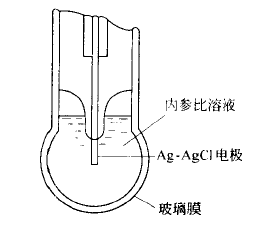
\includegraphics[width=0.4\linewidth]{image/chp7_glass_electrode}
	\caption{pH玻璃膜电极}
	\label{fig:chp7glasselectrode}
\end{figure}

产生电势的关键在玻璃膜,其内外的$\ce{H+}$浓差梯度导致了扩散电位的形成。若改变其成分,则可以响应不同离子的浓度差。

当[$\ce{Na+}$]浓度很大时,出现误差,称为钠差。修正电势大小为$E=K+0.0592\lg ( {\alpha_{\ce{H+},out}}+c\alpha^{1/n_j})$,$k_j$称为选择性系数,值越小,选择性越好。

玻璃电极本质上是一种离子选择性电极,现列举其他几种离子选择性电极:
\begin{itemize}
	\item $\ce{F-}$选择电极:$E=K-0.0592\lg {\alpha_{\ce{F-}}}$
	\item $\ce{Na+}$选择电极
	\item $\ce{Ca^2+}$选择电极
\end{itemize}

\subsubsection{酶电极}
酶电极(enzyme electrode)的分析原理是基于用电位法直接测量酶促反应中反应物
的消耗或反应物的产生而实现对底物分析的一种分析方法。它将酶活性物质覆盖在电极
表面,这层酶活性物质与被测的有机物或无机物(底物)反应,形成一种能被电极
响应的物质。
\begin{example}
	尿素在尿素酶催化下发生下面的反应:
	$$\ce{NH2CONH2 + 2H2O -> 2NH4+ + CO3^2-}$$
	反应生成的$\ce{NH4+}$可用铵离子电极来测定。若将
	尿素酶涂在铵离子选择电极上,则成为尿素电极,可测出待测液中尿素含量。
	
	葡萄糖氧化酶(葡萄糖酸)、氨基酸氧化酶($\ce{NH4+}$)也能做成酶电极。
\end{example}

\subsubsection{免疫电极}
抗体与抗原结合后的电化学性质与单一抗体或抗原的电化学性质有较大的差别。将抗体(或抗原)固定在膜或电极的表面,与抗原(或抗体)形成免疫复合物后,膜中电极表面的物理性质,如表面电荷密度、离子在膜中的扩散速度发生了改变,从而引起了膜电位或电极电位的改变。
\begin{example}
	将人绒毛膜促性腺激素(hCG)的抗体通过共价交联的方法固定在二氧化钛电
	极上,形成检测hCG的免疫电极。当该电极上hCG抗体与被测液中的hCG形成免疫复合物时,电极表面的电荷分布发生变化。该变化通过电极电位的测量检测出来。
\end{example}


\subsection{参比电极}

\begin{definition*}{参比电极}{}
	与被测物质无关的,提供测量电位参考的电极称为参比电极。
\end{definition*}

条件:
\begin{itemize}
	\item 能迅速建立热力学平衡电位,这就要求电极反应是可逆的;
	\item 电极电位是稳定的,能允许仪器进行测量。
\end{itemize}

常用的参比电极如表\ref{tab:canbidianji}所示。

\begin{table}[!h]
	\centering
	\caption{常用的参比电极}
	\small
	\begin{tabular}{ccc}
		\toprule
		参比电极  & {饱和甘汞电极} & {银/氯化银电极} \\
		\midrule
		电解液   & $\ce{KCl}$溶液 & $\ce{KCl}$溶液 \\
		电极反应  & $\ce{2Hg + 2Cl- - 2e- -> Hg2Cl2}$ & $\ce{Ag + Cl- - e- -> AgCl}$ \\
		电极电势  & $\varphi=\varphi^{\Theta}- 0.0592\ln a_{\ce{Cl-}}$ & $\varphi=\varphi^{\Theta}-0.0592\ln a_{\ce{Cl-}}$ \\
		\midrule
		优缺点    & \tabincell{c}{电势稳定、重现性好\\ 可以通过陶瓷塞/多孔玻璃与指示电极相连\\具有一定的阻抗和电流负载能力\\温度滞后性大,有毒性} & \tabincell{c}{电势稳定、重现性好\\ 容易制备,能在更高温度下使用\\体积小,可以很灵活\\ 在外参比溶液中应先加入\\$\ce{AgCl}$饱和,否则易溶解} \\
		\bottomrule
	\end{tabular}%
	\normalsize
	\label{tab:canbidianji}%
\end{table}%

\subsection{电位分析法测定pH值}

pH玻璃电极是测量氢离子活度最重要的指示电极,它和甘汞电极组成的体系是最常用的体系。溶液pH值的测量通常采用与已知pH值的标准缓冲溶液相比较的方法进行。对于$\mathrm{pH}$已知的标准缓冲溶液(s)和未知溶液(x),测得的电动势分别为
\begin{gather*}
	E_x=K+0.0592\lg {\alpha_{\ce{H+},x}}-E_{SCE}\\
	E_s=K+0.0592\lg {\alpha_{\ce{H+},s}}-E_{SCE}
\end{gather*}

其中$E_{SCE}$是饱和甘汞电极的电势。可以求得:
\begin{gather*}
	\mathrm{pH}=\mathrm{pH}_s-\dfrac{E_x-E_s}{0.0592}
\end{gather*}

有多组缓冲液时,还可以用标准曲线法。

该法适用于$\mathrm{pH}=1\sim 9$的情况。$\mathrm{pH}<1$时,读数偏低;$\mathrm{pH}>9$时,读数偏高。

\section{电解和库仑分析法}
%3、理解电解和库仑分析法。化学电池是电解池?什么是分解电压?

这一部分所用的化学电池是\textbf{电解池}。

\subsection{电解分析法}
\begin{definition*}{电解分析法}{}
	通过测量电解中沉积于电极表面的沉积物质量进行分析的一类方法。
\end{definition*}

\begin{example}
	现以电解0.5$\mathrm{mol/L}$\ $\ce{H2SO4}$和$\ce{CuSO4}$的混合溶液为例说明电解过程。
	
	\begin{itemize}
		\item 阴极:$\ce{Cu^2+ + 2e- -> Cu}$
		\item 阳极:$\ce{2H2O - 2e- -> O2 + 4H+}$
	\end{itemize}

	可以测量沉积于阴极表面的$\ce{Cu}$的质量,对溶液进行分析,如测量$\ce{Cu^2+}$浓度。
\end{example}

结合标准电极电势和能斯特方程可计算出阴阳极的实际电位$E_{\text{阴}},E_{\text{阳}}$。

\begin{definition*}{理论分解电压}{}
	\begin{equation*}
	E_{\text{分,理}}=E_{\text{阳}}-E_{\text{阴}}
	\end{equation*}
\end{definition*}

但由于$iR$降(克服电解质溶液的电阻)、过电位(阴阳极的极化现象),使电解发生所需的实际电压要高于$E_{\text{分,理}}$。

\begin{definition*}{(实际)分解电压\footnote{未考虑液体接界电位$E_j$}}{}
	\begin{equation*}
	E_{\text{分}}=E_{\text{分,理}}+iR+\eta_{\text{阳}}-\eta_{\text{阴}}
	\end{equation*}
\end{definition*}

其中
\begin{itemize}
	\item $i$为电解电流,$R$为电解回路总电阻;
	\item $\eta_{\text{阳}},\eta_{\text{阴}}$分别是阳极、阴极的超电位,即电极电位与可逆电极电位的差值。
\end{itemize}

\begin{note}
	电极极化:是指电流流过电极时,电极电位偏离可逆电极电位的现象。可分为:
	\begin{itemize}
		\item 浓差极化:由于电解过程中电极表面附近的溶液浓度与本体浓度的差异引起的,使正极电位增大,负极电位减小。
		
		减小浓差极化的方法:增大电极面积、减小电流密度、强化机械搅拌。
		\item 电化学极化:电极反应速度慢,电极上聚集了一定的电荷。阴极聚集过多正电,使电极电位减小;反之增大。
	\end{itemize}
\end{note}


电解分析的主要类别有:
\begin{definition*}{控制电位电解分析}{}
	工作电极的电位控制在某一合适的电位值或某一个小范围内,使被测离子在工作电极上析出,其它离子则留在溶液中,以达到{\heiti 分离和测定}的目的。
\end{definition*}

\begin{example}
	电解1$\mathrm{mol/L}$$\ce{Cu^2+}$和0.01$\mathrm{mol/L}$$\ce{Ag+}$的混合溶液。
	
	\begin{itemize}
		\item $E_{\ce{Cu^2+}}=0.337\mathrm{V}$
		\item $E_{\ce{Ag+}}=0.681\mathrm{V}$,故银先析出
		\item 当$c_{\ce{Ag+}}=10^{-6}\mathrm{mol/L}$时,$E_{\ce{Ag+}}=0.445\mathrm{V}$,铜仍不会析出,故能分离两种离子。
	\end{itemize}
	
	可以测量沉积于阴极表面的$\ce{Cu}$的质量,对溶液进行分析,如测量$\ce{Cu^2+}$浓度。
\end{example}

恒电流电解分析、汞阴极电解分析的例子在课本上,不确定是否考,暂未列入。

\subsection{库仑分析法}
\begin{definition*}{库仑分析法}{}
	通过测量电解中消耗的电量进行分析的一类方法。
\end{definition*}
	
\begin{theorem*}{基本公式}{}
	\begin{gather*}
	m=\dfrac{MQ}{nF}\\
	Q=\int i\di{t}
	\end{gather*}
	
	其中$m$为析出的物质的量,$M$为该物质的相对量,$n$为电极反应电子数,$Q$为通过的总电荷量。
\end{theorem*}

库仑分析法主要分为:

\begin{itemize}
	\item 控制电位库仑分析:通过库仑计求出电量$Q$,直接计算。
	\item 恒电流库仑分析:控制电解电流一定,又称库仑滴定法。
\end{itemize}
%怎么恒电流的还没清楚

\begin{example}
	恒电流库仑分析:测$\ce{AsO3^3-}$含量。在一定浓度的$\ce{H2SO4}$介质、$\ce{KBr}$辅助电解质中,
	
	\begin{itemize}
		\item 阴极:$\ce{2H+ + 2e- -> H2 ^ }$
		\item 阳极:$\ce{2Br- - 2e- -> Br2}$
	\end{itemize}

	电解产生的$\ce{Br2}$立即氧化$\ce{AsO3^3-}$:
	
	$\ce{AsO3^3- + Br2 + H2O -> AsO4^3- + 2Br- + 2H+}$
	
	恢复了电极反应的物质,所以电动势不变,电流也不变,直到$\ce{AsO3^3-}$耗尽,电流计指针偏转指示终点。此法叫死停终点法\footnote{常用于氧化还原滴定体系,特别是以电生卤素为滴定剂的库仑滴定中应用最广。}。
\end{example}


\section{伏安分析法}
%4、了解极谱、伏安分析法?什么是极限扩散电流?什么是半波电位?

伏安分析法(voltammetry)是指以被分析溶液中电极的电压-电流行为为基础的一类电化学分析方法。与电位分析法不同,伏安分析法是在一定的电位下对体系电流的测量。

\subsection{极谱分析法}
\begin{definition*}{极谱分析法}{}
	采用滴汞电极的伏安分析法。
\end{definition*}

\begin{itemize}
	\item 阴极(指示电极):滴汞电极。电极表面仅有能斯特扩散层,从而产生了极谱分析所必需的浓差极化条件。
	\item 阳极(参比电极):甘汞电极。表面积大,电流密度小,电位稳定。
	\item 优势:汞滴可不断更新;氢的超电势很大,金属离子与$\ce{Hg}$生成汞齐,便于析出。
	\item 局限:汞对环境的污染、对人体的伤害;存在充电电流,现在有许多改进。
\end{itemize}

\begin{note}
	极谱分析的充电电流:当无电压时,甘汞电极带正电,滴汞电极不带电,甘汞电极向滴汞电极充电,产生充电电流,与电解方向相反,为负充电电流。当电压很大时,甘汞电极带负电,形成正充电电流。充电电流是是提高灵敏度的障碍。
\end{note}

\begin{example}
	以测$\ce{Cd^2+}$离子浓度为例说明其原理。
	
	\begin{itemize}
		\item 阴极:$\ce{Cd^2+ + 2e- -> Cd}$
		\item 阳极:$\ce{2Hg + 2Cl- - 2e- -> Hg2Cl2}$
	\end{itemize}

	逐渐增大外加电压,测量电流值。
	
	\begin{itemize}
		\item 电压很小,未达到$E_{\text{分}}$时,只有残余(背景)电流$i_r$。
		\item 开始析出金属后,电流随电压的增大而增大。
		\item 可以想象,当电压增大到一定程度,反应速率很快,以致电极周围的$\ce{Cd^2+}$被迅速消耗,此时需要周围溶液补充$\ce{Cd^2+}$,补充的快慢取决于离子的扩散速率。扩散速率决定了反应速率(即电流)的上限。
	\end{itemize}

	典型的极谱图如图\ref{fig:chp7jipufenxiivfigure}。
\end{example}

\begin{figure}[!h]
	\centering
	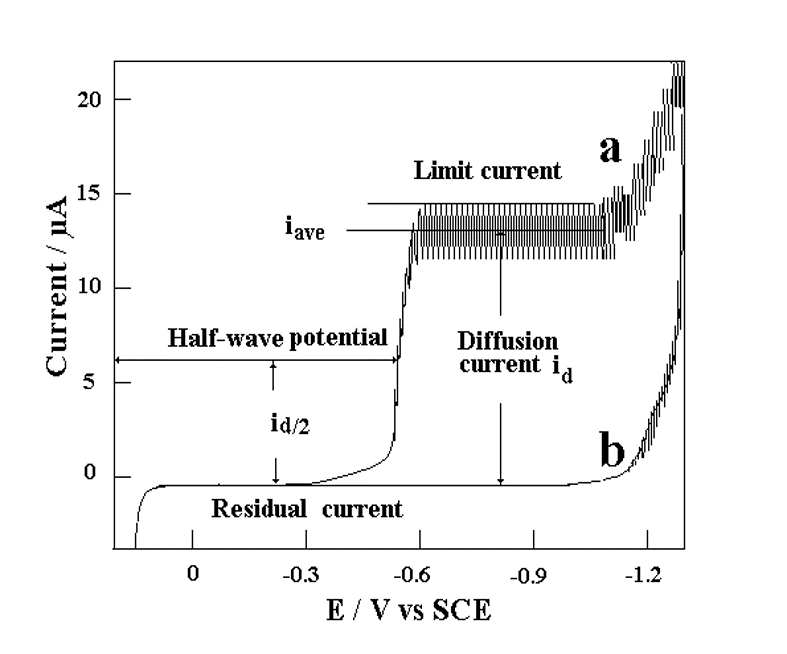
\includegraphics[width=0.7\linewidth]{image/chp7_jipufenxi_IVfigure}
	\caption{极谱图}
	\label{fig:chp7jipufenxiivfigure}
\end{figure}

由此可以引出概念:

\begin{definition*}{极限扩散电流}{}
	扩散电流是指在极谱分析中由溶液本体扩散到电极表面的金属离子所形成的电流。
	
	当扩散速率达到最大时所形成的电流就称为极限扩散电流。即图中的$i_d=i_{ave}-i_r$
\end{definition*}
%没写和浓度成正比那个

不过一般$i_r$较小,若不是分析微量组分时影响不大。

\begin{theorem*}{尤可维奇方程}{}
	\begin{equation*}
		i_{d,ave}=607nD^{\frac{1}{2}}m^{\frac{2}{3}}t^{\frac{1}{6}}c
	\end{equation*}
	
	$D$为扩散系数,$m$为汞滴的流速,$t$为汞滴的寿命。
	
	$h$为汞柱的高度,毛细管常数$m^{\frac{2}{3}}t^{\frac{1}{6}}\propto h^{\frac{1}{2}}$。
\end{theorem*}

所以实验条件相同时,$i_{d,ave}\propto c$,可以用标准曲线法测样品浓度。

\begin{note}
	影响扩散电流的因素:
	\begin{itemize}
	\item 残余电流:杂质的法拉第电流,电容电流;
	\item 极谱极大:电流变平稳之前有一个峰,如图\ref{fig:chp7jipujida};
	\item 毛细管特性:见上。实验过程中$h$应该保持一致。
	\item 滴汞电极电位:$t$受滴汞与溶液界面的表面张力$\gamma$影响。
	\item 温度:对扩散系数$D$有显著影响,电解池内溶液的温度波动应控制在$0.5$\textcelsius 以内。
	\item 溶液组成:引起溶液粘度的变化,扩散电流与粘度系数成反比。
	\item 氧波:溶解氧参与电极反应。
	\end{itemize}
\end{note}

\begin{figure}[!h]
	\centering
	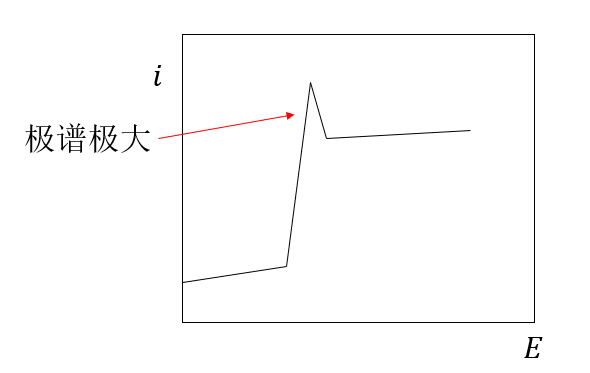
\includegraphics[width=0.5\linewidth]{image/chp7_jipujida}
	\caption{极谱极大}
	\label{fig:chp7jipujida}
\end{figure}

\begin{note}
	消除误差的方法:
	\begin{itemize}
		\item 减小电容电流:减小电极表面积;
		\item 消除迁移电流:加支持电解质,使池内阻变小,电压降低。
		\item 消除对流电流:不搅拌。
		\item 消除氧波:通入惰性气体,把溶解在水中的氧气驱除。
		\item 消除极谱极大:加入表面活性剂,如明胶等。
	\end{itemize}
\end{note}

\begin{definition*}{半波电位}{}
	在极谱曲线半峰高处的电位称为半波电位,即$i=i_r+i_d/2$处的电位。
	
	对于可逆波,物质的氧化半波电位与该物质的还原半波电位相同。	
\end{definition*}

半波电位只与离子本性有关,与浓度无关,是离子的特性常数,可作为定性分析的基础。在实际工作中,半波电位主要应用于分析实验条件的选择,以防止共存离子的干扰。

\subsection{循环伏安法}
如果以三角波电位进行扫描,所获得的电流响应与电位信号的关系称为循环伏安扫描曲线。
\begin{figure}[!h]
	\centering
	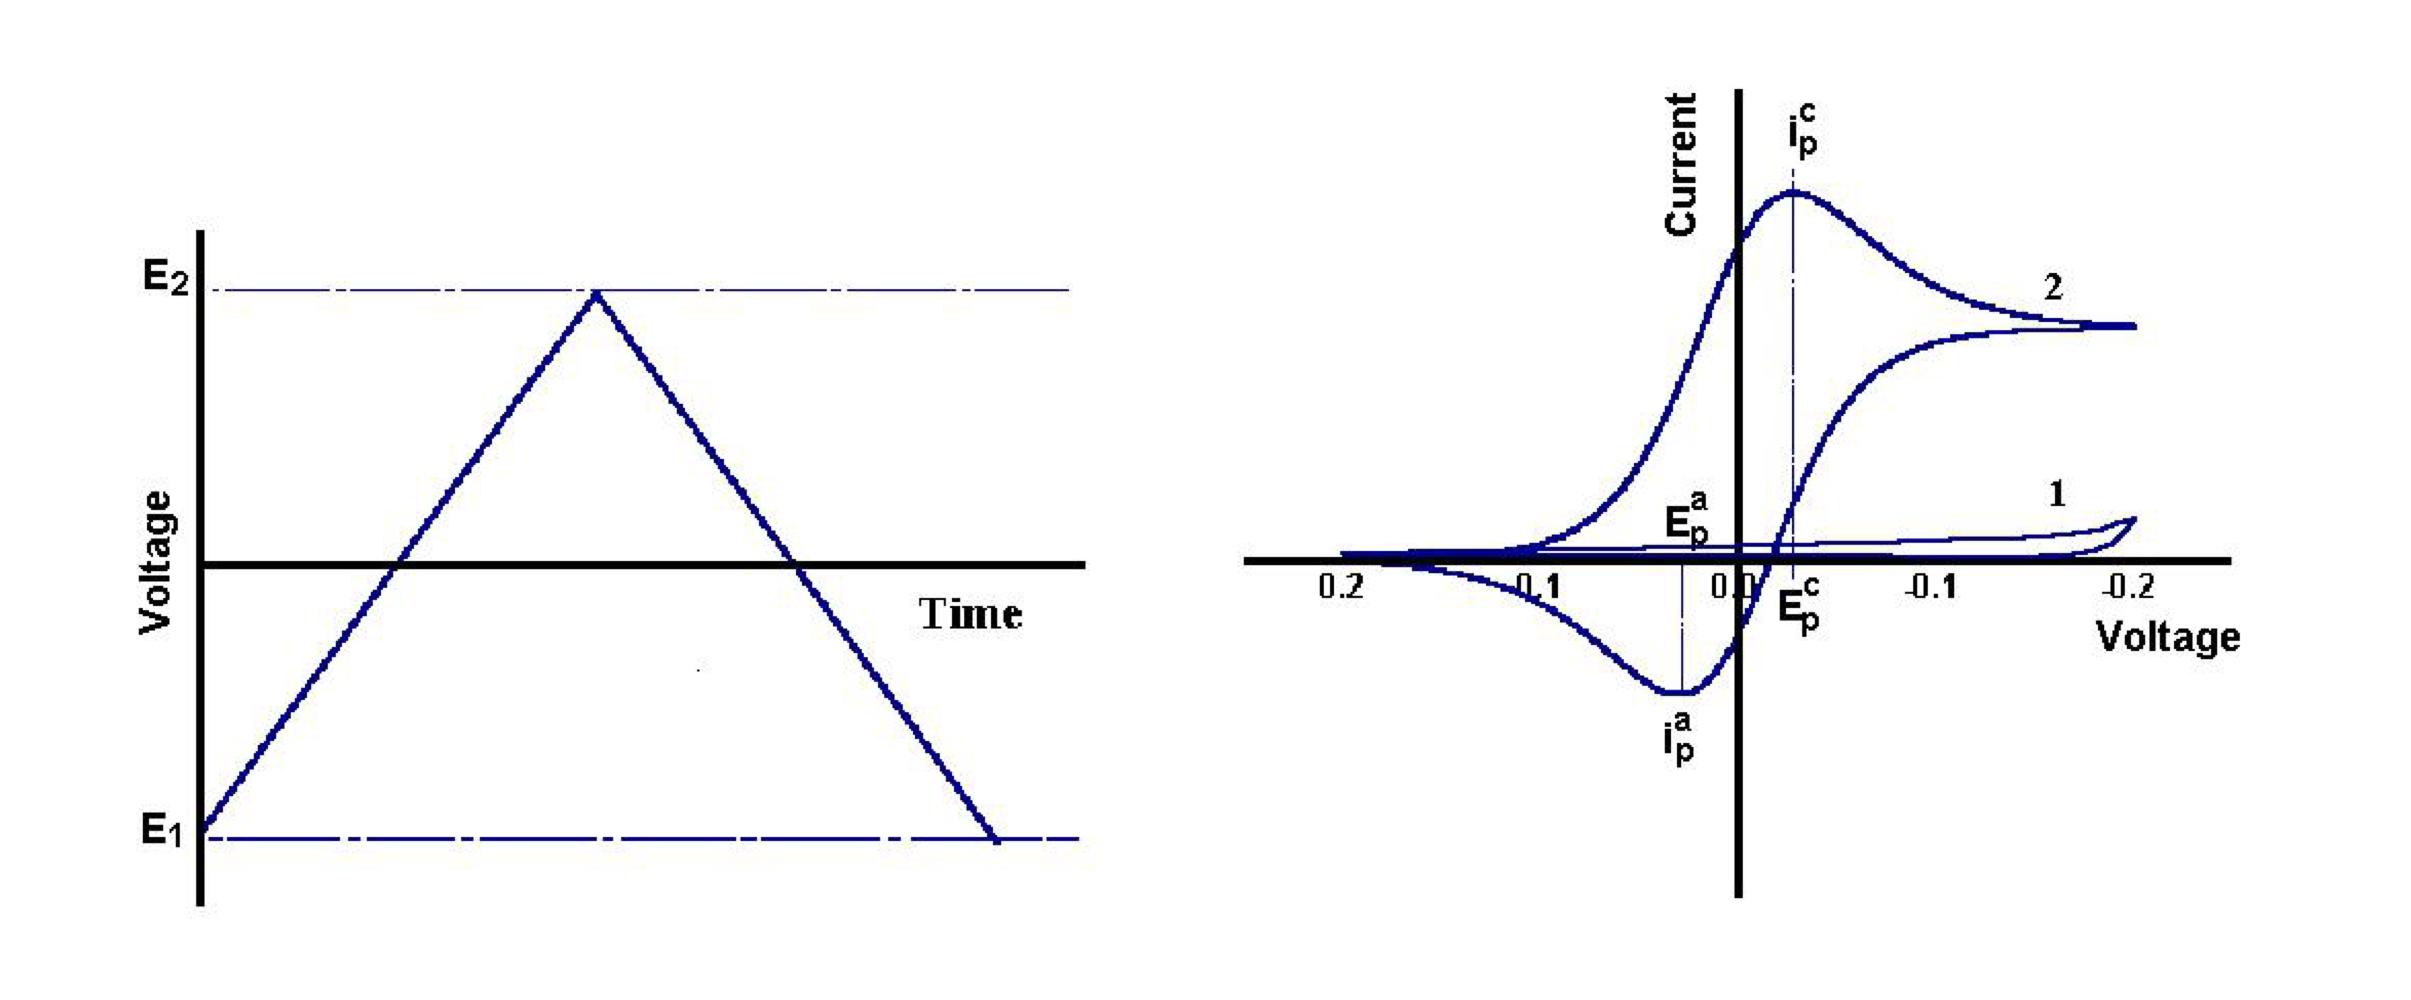
\includegraphics[width=0.9\linewidth]{image/chp7_circular_VA}
%	\caption{}
	\label{fig:chp7circularva}
\end{figure}

正向扫描时,电位从$E_1$扫到$E_2$,电位辐值为$0.4\mathrm{V}$,反扫时电位从$E_2$到$E_1$。$E_p^c,E_p^a$分别代表阴极峰值电位和阳极峰值电位。$I_p^c,I_p^a$分别代表阴极峰值电流和阳极峰值电流。(p代表峰值,a代表阳极,c代表阴极)。

\begin{example}
	\begin{figure}[!h]
		\centering
		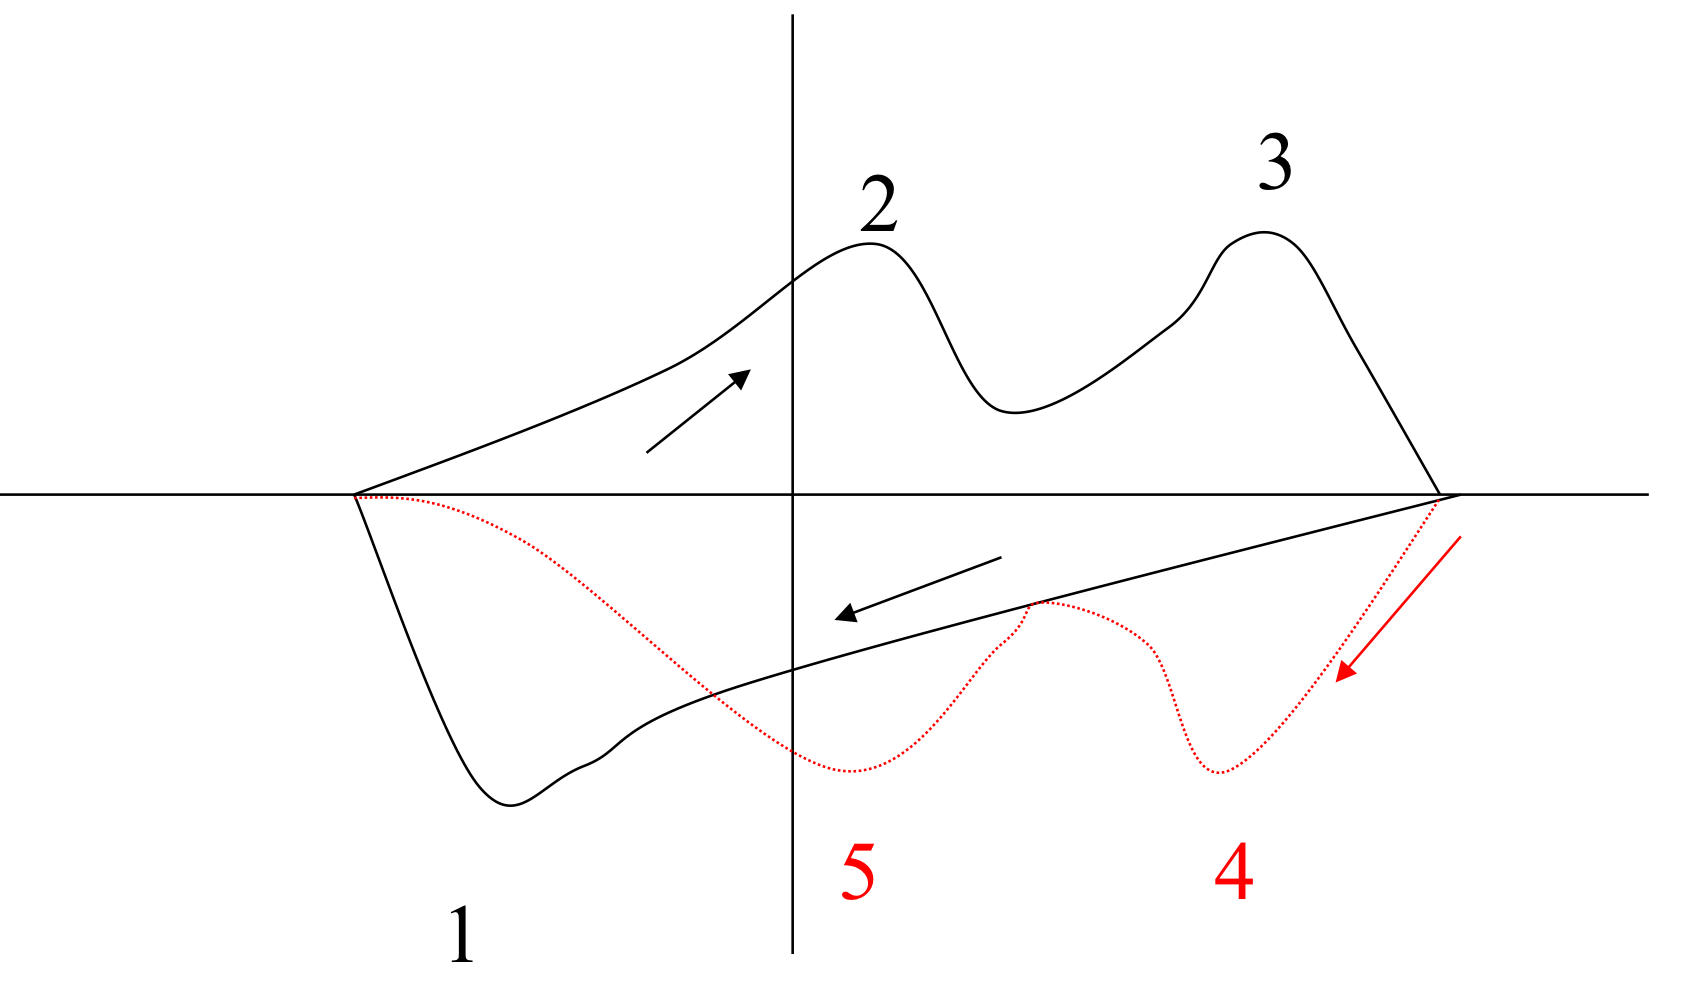
\includegraphics[width=0.7\linewidth]{image/chp7_circular_VA_example}
		\caption{}
		\label{fig:chp7circularvaexample}
	\end{figure}

	图\ref{fig:chp7circularvaexample}中的几个信号分别对应以下反应:
	
	\begin{figure}[!h]
		\centering
		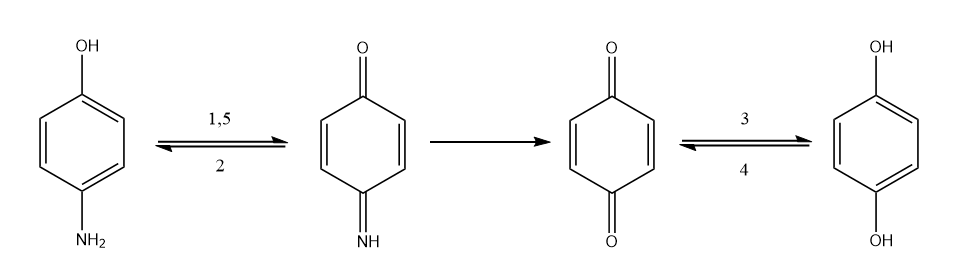
\includegraphics[width=\linewidth]{image/chp7_circular_VA_example_result}
%		\caption{}
		\label{fig:chp7circularvaexampleresult}
	\end{figure}
	
	参考:\url{https://wenku.baidu.com/view/df58d5d309a1284ac850ad02de80d4d8d15a01f2.html}
\end{example}
循环伏安分析方法可用于研究氧化还原体系的反应粒子浓度以及该体系的电化学性质,如血红蛋白、细胞色素C。
